\documentclass[tikz]{standalone}
\usepackage{tikz}
\usetikzlibrary{positioning, graphs}
\usetikzlibrary{graphs.standard}
\begin{document}
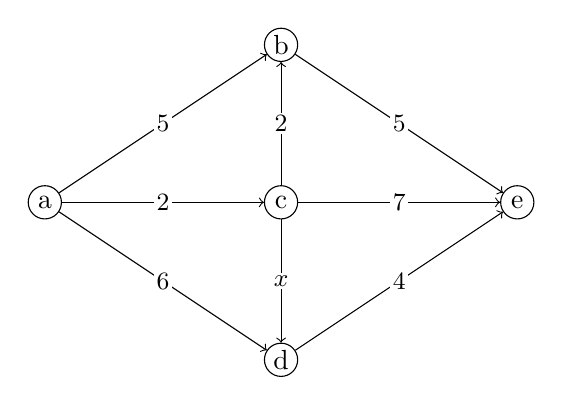
\begin{tikzpicture}
\begin{scope}
		[vertex/.style={draw,circle,inner sep = 0em, minimum size = 1.2em},
		 edgelabel/.style = {fill = white, inner sep = 0.1em, font=\small}]
		\node[vertex] (a) at (0,0) {a};
		\node[vertex] (b) at (3,2) {b};
		\node[vertex] (c) at (3,0) {c};
		\node[vertex] (d) at (3,-2) {d};
		\node[vertex] (e) at (6,0) {e};
		
		\draw[->] (a) to node[edgelabel] {$5$} (b);
		\draw[->] (a) to node[edgelabel] {$2$} (c);
		\draw[->] (a) to node[edgelabel] {$6$} (d);
		\draw[->] (b) to node[edgelabel] {$5$} (e);
		\draw[->] (c) to node[edgelabel] {$2$} (b);
		\draw[->] (c) to node[edgelabel] {$x$} (d);
		\draw[->] (c) to node[edgelabel] {$7$} (e);
		\draw[->] (d) to node[edgelabel] {$4$} (e);
\end{scope}
\end{tikzpicture}
\end{document}